	\begin{Huge}
			Informatik (Bachelor of Education)
		\end{Huge}
		\begin{exampleblock}{\textcolor{white}{Was ist der Studiengang?}}
			
		\end{exampleblock}
	
	\begin{block}{Welcher Teil macht wie viel im Studium aus?}
		\begin{figure}[h!]
			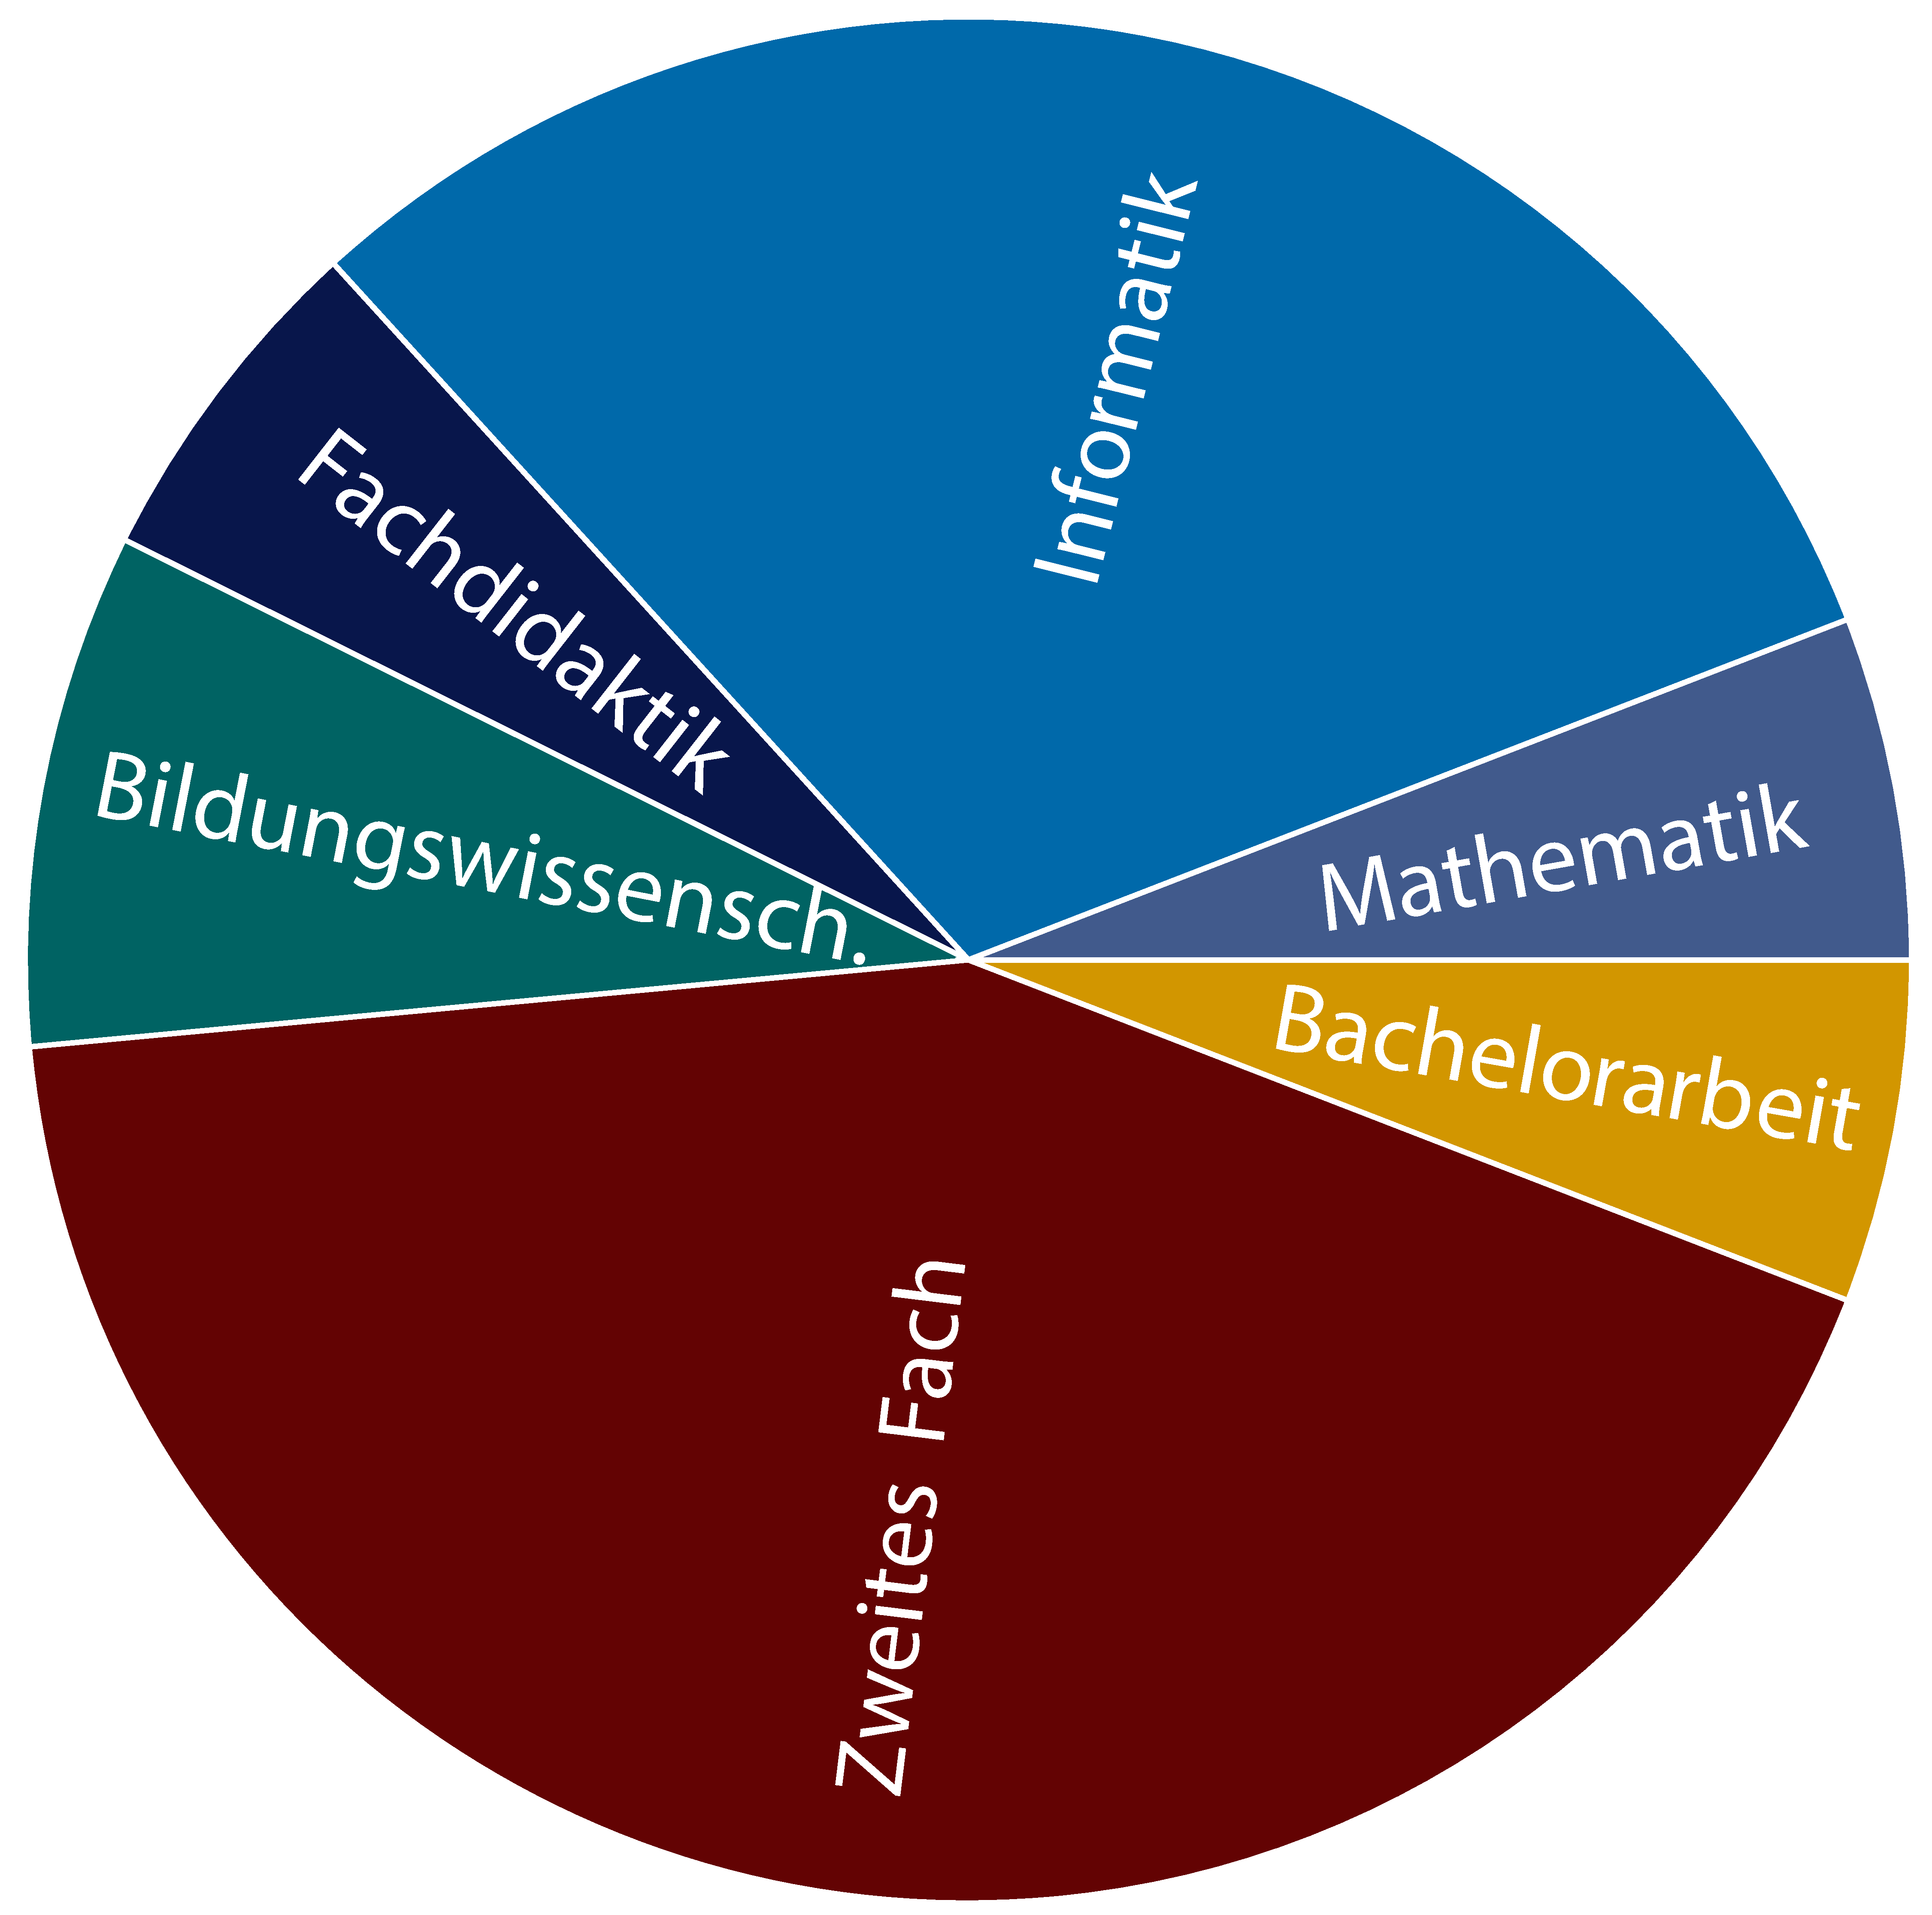
\includegraphics[width=0.4\textwidth]{charts/lehramt_informatik_piechartonly.pdf}
			\caption{Verteilung der Themenbereiche über das komplette Studium}
		\end{figure}
	\end{block}
	
	\begin{block}{Was macht man in welchem Semester?}
		\begin{figure}[h!]
			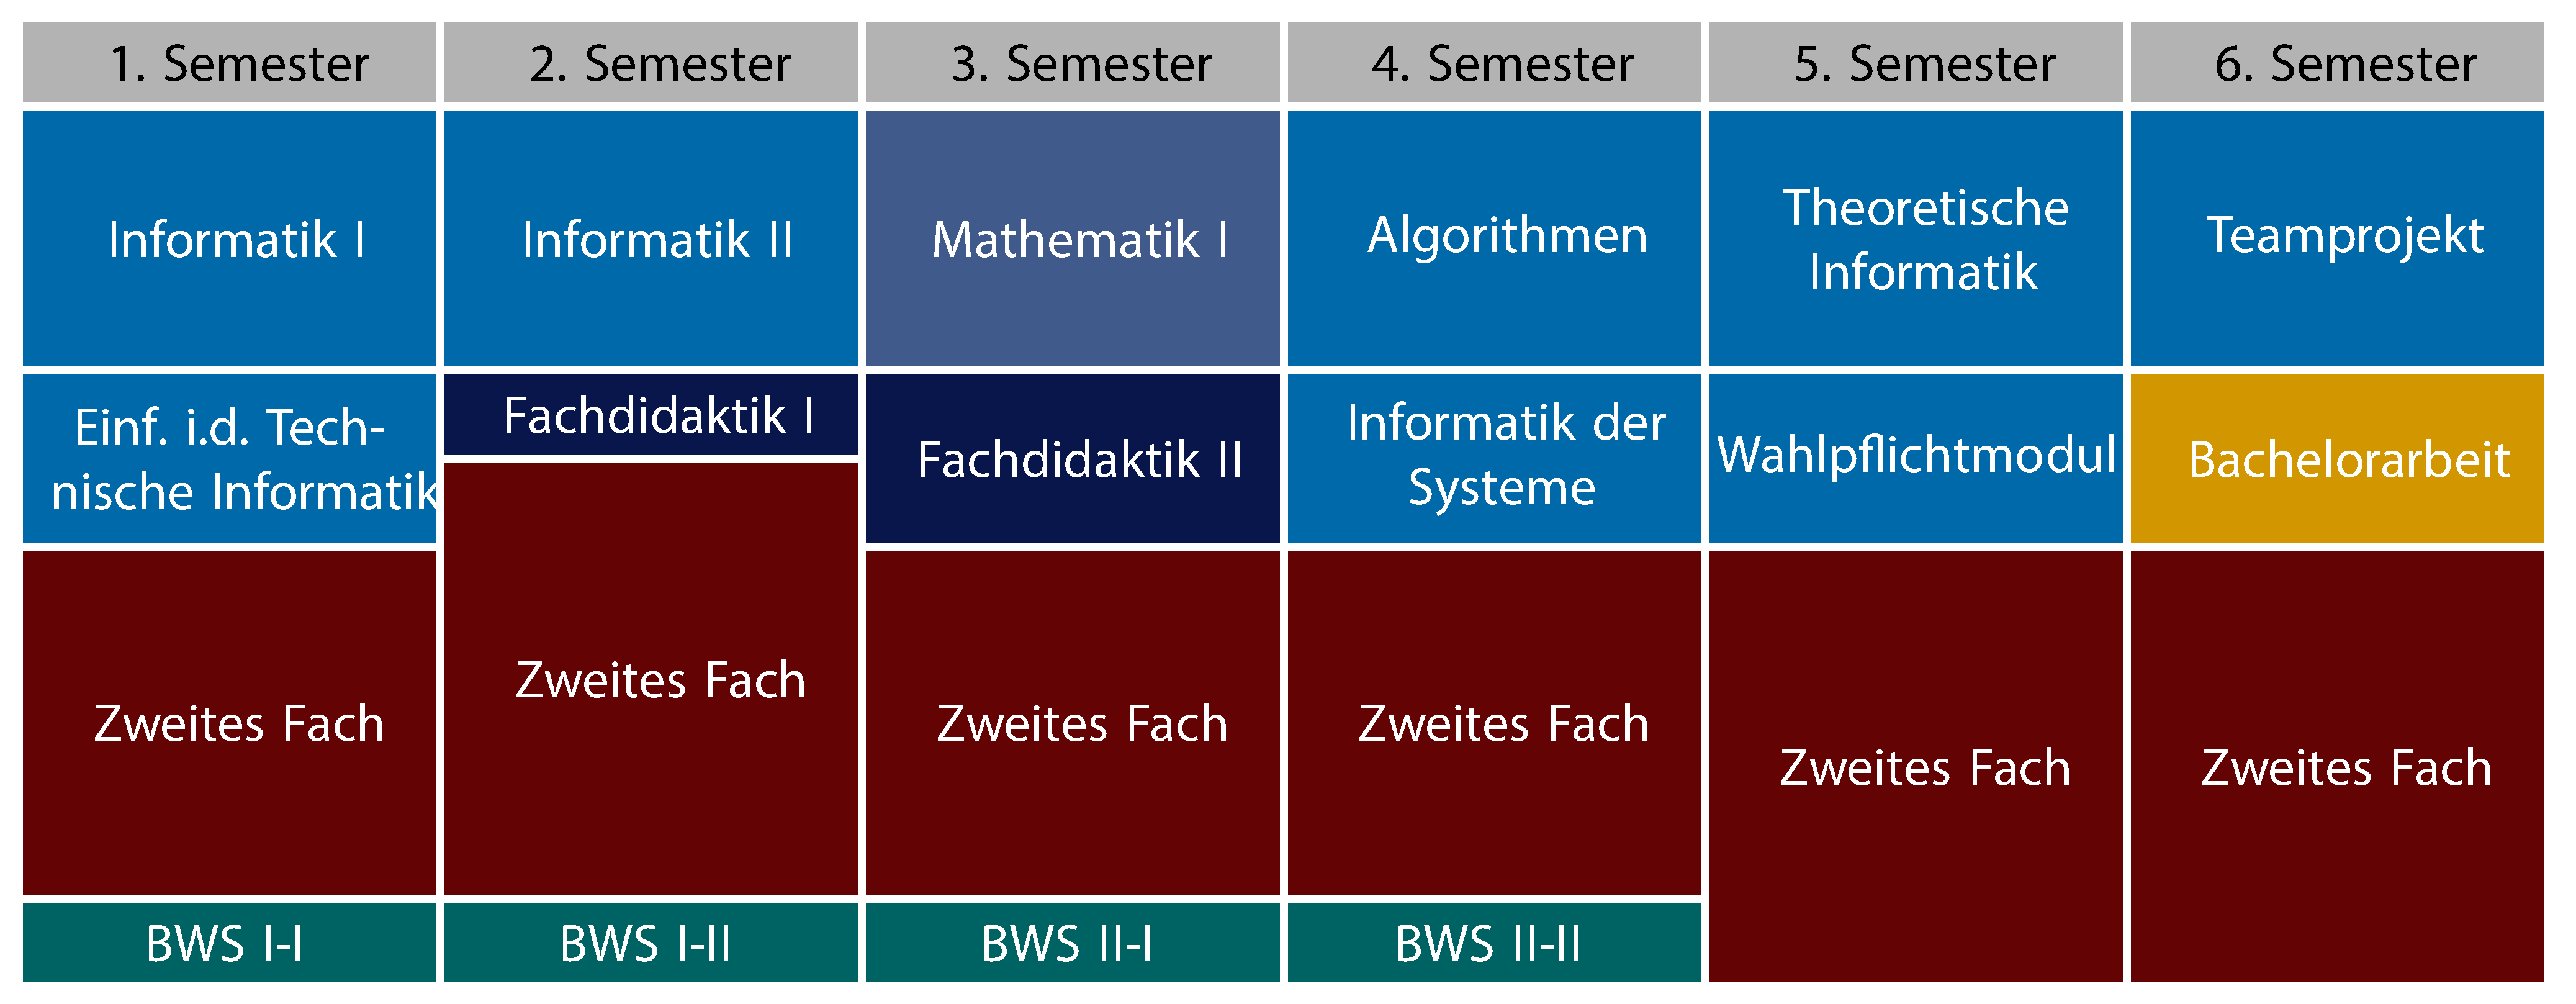
\includegraphics[width=\textwidth]{charts/lehramt_informatik_Studienplanonly.pdf}
		\end{figure}
		Das 1. Semester ist nach Plan ein Wintersemester, der Studienbeginn ist hier auch nur zum Wintersemester möglich. 
		Dieser Verlauf ist lediglich ein Vorschlag und kein bindender Studienplan. Es empfiehlt sich jedoch, den Plan einzuhalten, wenn man in Regelstudienzeit studieren möchte.
	\end{block}
\vfill
\begin{flushright}
	
\includegraphics[width=0.4\textwidth]{fsilogo.pdf}
\end{flushright}